\documentclass[11pt,a4paper]{article}
\usepackage[margin=1in]{geometry}
\usepackage[T1]{fontenc}
\usepackage{lmodern}
\usepackage{microtype}
\usepackage{amsmath,amssymb}
\usepackage{graphicx}
\usepackage{booktabs}
\usepackage{multirow}
\usepackage{array}
\usepackage{xcolor}
\usepackage[font=small,labelfont=bf]{caption}
\usepackage{subcaption}
\usepackage[ruled,vlined,linesnumbered]{algorithm2e}
\usepackage{tikz}
\usepackage[section]{placeins}
\usetikzlibrary{arrows.meta,positioning}
\usepackage[numbers,sort&compress]{natbib}
\usepackage[colorlinks=true,linkcolor=blue!50!black,citecolor=blue!50!black,urlcolor=blue!50!black]{hyperref}
\usepackage[capitalise,noabbrev]{cleveref}
\graphicspath{{../figures/}}
\newcommand{\tabdir}{../tables/en}
\newcommand{\pct}{\,\%}
\setlength{\emergencystretch}{2em}

\title{\textbf{Does Dynamics-Informed Imputation Transfer to Solar PV?}\\[2pt]
\large An Empirical Evaluation of Full-Partial Reconstruction Mapping on Real Photovoltaic Data}
\author{Jongkyu Kim\thanks{Corresponding author: \href{mailto:jk.kim@60hz.io}{jk.kim@60hz.io}}\\\small\href{mailto:jk.kim@60hz.io}{jk.kim@60hz.io}
\and Claude Opus 5.5\thanks{AI system (Anthropic). See the AI disclosure statement at the end of the paper.}}
\date{October 2026}

\begin{document}
\maketitle

\begin{abstract}
Gaps in photovoltaic (PV) monitoring data are routine and costly, yet most gap-filling practice relies on interpolation or neighbour scaling.
Full-Partial Reconstruction Mapping (FPRM), recently proposed by Wu et al.\ (Nature Communications, 2026), imputes an incomplete time series by learning, with Gaussian process regression, a map from the delay-coordinate reconstruction of a fully observed series to the incomplete one, and reports reliable recovery even at 90\pct{} missingness.
We test whether this dynamics-informed approach transfers to solar PV.
We re-implement FPRM, reproduce the paper's benchmark on a low-dimensional ecological system, and evaluate it on four fully observed NREL PVDAQ datasets (three sites, hourly and 15-min, 4--10 series each) under seven realistic missingness mechanisms, against 13 baselines and several FPRM variants (480 main test sets plus 134 ablation test sets).
Delay embedding transfers: relative to the same model without embedding, it lowers daytime RMSE by a median 7\pct{} and helps for every one of 31 reference choices.
However, the paper's single-reference FPRM is 12--16\pct{} worse than the best per-test-set baseline in ordinary gap scenarios, typically random forests or SVR on all complete neighbours; an extension that embeds all complete references (FPRM-multi) narrows the gap to 5--9\pct{} and attains the best mean rank of 17 methods.
FPRM is clearly superior only in the regime the original paper emphasises (one complete series, 90\pct{} missing elsewhere: 5--14\pct{} better on all four datasets), and it fails under missing-not-at-random peak loss, time-of-day-aliased logging and region-wide outages.
We conclude that FPRM is a conditionally useful specialist tool for PV data, and we give concrete guidance on reference selection and learner choice.
\end{abstract}

\noindent\textbf{Keywords:} missing data imputation; photovoltaics; delay embedding; Takens' theorem; Gaussian process regression; benchmark

\section{Introduction}\label{sec:intro}

Operational PV fleets produce long multivariate time series of inverter output, meter readings and on-site irradiance.
These series are routinely interrupted by communication failures, logger outages, low-rate polling, sensor saturation and site-wide power loss.
Gaps bias energy accounting, performance-ratio estimates, degradation analysis and the training of forecasting models, so imputation is a practical necessity.
In practice it is usually done with linear interpolation, clear-sky-index interpolation or scaling of a neighbouring system.

Wu et al.~\cite{wu2026fprm} recently proposed \emph{Full-Partial Reconstruction Mapping} (FPRM), a dynamics-informed imputation framework grounded in Takens' embedding theorem~\cite{takens1981,deyle2011}.
For every incomplete series, FPRM reconstructs the attractor of the underlying system from the delay coordinates of a fully observed series (the \emph{full reconstruction}) and from the incomplete series itself (the \emph{partial reconstruction}).
It then learns the diffeomorphic map between them with Gaussian process regression (GPR).
On model systems and on traffic, EEG, exchange-rate and wind data, FPRM reportedly recovers series with up to 90\pct{} missing values and outperforms statistical, machine-learning and dynamics-aware baselines~\cite{wu2026fprm}.

PV output is an attractive but non-trivial target for this idea.
On one hand, neighbouring systems are driven by the same cloud field, so a complete neighbour plausibly carries the state information that FPRM exploits.
On the other hand, PV output is dominated by a deterministic diurnal forcing, is exactly zero at night, saturates at inverter limits, and is often missing for reasons correlated with its value.
None of these properties is typical of the autonomous chaotic systems used to motivate FPRM.
We therefore ask three questions:
\begin{enumerate}
  \item Under realistic PV missingness mechanisms, does FPRM beat simple PV practice (interpolation, neighbour scaling) and general-purpose machine-learning imputers?
  \item Under which conditions (missing ratio, gap structure, type of reference series, temporal resolution) does it succeed or fail?
  \item What settings and limitations should a practitioner be aware of?
\end{enumerate}

\paragraph{Contributions.}
\begin{itemize}
  \item An open Python re-implementation of FPRM with observed-data-only selection of embedding parameters. It reproduces the paper's low-dimensional ecology benchmark (\cref{sec:synthetic}).
  \item A PV imputation benchmark built from four fully observed NREL PVDAQ windows~\cite{pvdaq} and eight missingness scenarios (S1--S8), covering random, block, whole-day, periodic, threshold (MNAR), single-reference, simultaneous and reference-choice settings (\cref{sec:setup}).
  \item A comparison of FPRM, its ablations and 13 baselines on 614 test sets with paired significance tests (\cref{sec:results}).
  \item Evidence that delay embedding helps on PV data, but that the paper's single-reference design discards information that standard regressors exploit. An all-reference extension (FPRM-multi) closes most of the gap.
  \item Practical guidance: prefer the best-correlated neighbouring \emph{output} series over an irradiance sensor as reference; use SVR instead of GPR (same accuracy, $\sim$45$\times$ faster); and route gaps by missingness pattern (\cref{sec:discussion}).
\end{itemize}

\section{Related work}\label{sec:related}

\paragraph{Missing-data theory and generic imputers.}
Missingness mechanisms are classified as missing completely at random (MCAR), at random (MAR) or not at random (MNAR)~\cite{rubin1976,little2019}.
Widely used generic imputers include chained-equation imputation (MICE)~\cite{vanbuuren2011}, $k$-nearest-neighbour imputation~\cite{troyanskaya2001} and random-forest imputation~\cite{breiman2001,stekhoven2012}.
Deep generative and recurrent imputers such as GAIN~\cite{yoon2018gain}, BRITS~\cite{cao2018brits} and SAITS~\cite{du2023saits} learn temporal and cross-series structure from large training sets.
We include MICE and $k$NN imputation as multivariate baselines and leave deep imputers to future work (\cref{sec:limitations}).

\paragraph{State-space reconstruction.}
Takens' theorem~\cite{takens1981} and its multivariate generalisation~\cite{deyle2011} guarantee that delay coordinates of a single observable can reconstruct an attractor that is diffeomorphic to the original.
Embedding parameters are classically chosen with the first minimum of the auto mutual information~\cite{fraser1986} and the false-nearest-neighbour criterion~\cite{kennel1992}.
Empirical dynamic modelling builds on this: S-map~\cite{sugihara1994} performs locally weighted linear prediction in the reconstructed space, convergent cross mapping~\cite{sugihara2012} uses it to infer causality, and multiview embedding (MVCM)~\cite{ye2016} combines many embeddings.
FPRM~\cite{wu2026fprm} departs from these neighbour-based methods by learning a global map between full and partial reconstructions with GPR~\cite{rasmussen2006}.

\paragraph{PV data.}
Clear-sky models such as Ineichen--Perez~\cite{ineichen2002}, available in pvlib~\cite{holmgren2018pvlib}, are the standard tool for normalising PV and irradiance series.
The clear-sky index and neighbour-ratio scaling are the de facto practitioner baselines for PV gap filling, and we include both.
To our knowledge, dynamics-informed imputation has not been evaluated on PV data with controlled, realistic missingness.

\section{Method}\label{sec:method}

\subsection{Full-Partial Reconstruction Mapping}

Let $x_i(t)$, $t=1,\dots,l$, be a fully observed series and $x_j(t)$ an incomplete one.
For embedding dimension $E$ and lag $\tau$, the full reconstruction is
\begin{equation}
  \mathbf{X}_i(t) = \big(x_i(t),\,x_i(t+\tau),\,\dots,\,x_i(t+(E-1)\tau)\big),\qquad t = 1,\dots,m,\; m = l-(E-1)\tau ,
  \label{eq:full}
\end{equation}
and the partial reconstruction $\mathbf{X}_j(t)$ is defined analogously from $x_j$, with missing coordinates.
By Takens' theorem both reconstructions are diffeomorphic to the system attractor $M$ ($f:M\to M(x_i)$, $g:M\to M(x_j)$).
Hence there is a smooth map $F = g\circ f^{-1}: M(x_i)\to M(x_j)$.
FPRM learns its first coordinate,
\begin{equation}
  x_j(t) = F\big(\mathbf{X}_i(t)\big),
  \label{eq:map}
\end{equation}
from the time points where $x_j(t)$ is observed, and imputes $\hat x_j(k) = F(\mathbf{X}_i(k))$ at the missing $k$~\cite[Eqs.~11--14]{wu2026fprm}.

$F$ is a GP with squared-exponential kernel $q(\mathbf{x},\mathbf{x}') = \exp\!\big(-\lVert\mathbf{x}-\mathbf{x}'\rVert^2/2\theta^2\big)$, whose scale $\theta$ is initialised to the mean predictor standard deviation, plus Gaussian noise $\sigma^2$.
The posterior mean is
\begin{equation}
  u_*(\tilde{\mathbf{x}}) = u(\tilde{\mathbf{x}}) + q(\tilde{\mathbf{x}},\mathbf{X})\,\big(q(\mathbf{X},\mathbf{X})+\sigma^2 I\big)^{-1}\big(\mathbf{y}-u(\mathbf{X})\big),
  \label{eq:gp}
\end{equation}
where $u$ is a constant mean~\cite[Eqs.~15--18]{wu2026fprm}.
Every incomplete series receives its own map; \cref{fig:pipeline} summarises the procedure.

\begin{figure}[t]
  \centering
  \newcommand{\PLa}{\textbf{complete series} $x_i$}
  \newcommand{\PLb}{\textbf{incomplete series} $x_j$}
  \newcommand{\PLc}{\textbf{full reconstruction}}
  \newcommand{\PLd}{\textbf{training pairs}}
  \newcommand{\PLe}{\textbf{learn mapping} $F$}
  \newcommand{\PLf}{\textbf{impute}}
  \newcommand{\PLg}{delay embed}
  \newcommand{\PLh}{missing $k$}
  \resizebox{\linewidth}{!}{% FPRM pipeline schematic (shared by en/ko; labels passed via macros \PLa ... \PLh)
\begin{tikzpicture}[
  font=\footnotesize, >=Stealth,
  box/.style={draw=black!60, rounded corners=2pt, fill=#1, align=center, minimum height=1.05cm, inner sep=3pt},
  box/.default=white]
  \definecolor{cblue}{HTML}{2a78d6}\definecolor{corange}{HTML}{eb6834}\definecolor{cgray}{HTML}{f0efec}
  % reference series
  \node[box=cblue!8, text width=2.6cm] (ref) at (0,0) {\PLa\\[2pt]
    \begin{tikzpicture}[x=0.22cm,y=0.22cm]\draw[cblue,thick] plot[smooth] coordinates {(0,0)(1,1.4)(2,2.1)(3,1.5)(4,0.3)(5,0)(6,1.2)(7,2.2)(8,1.6)(9,0.2)};\end{tikzpicture}};
  % incomplete series
  \node[box=corange!8, text width=2.6cm] (tgt) at (0,-2.3) {\PLb\\[2pt]
    \begin{tikzpicture}[x=0.22cm,y=0.22cm]\draw[corange,thick] plot[smooth] coordinates {(0,0)(1,1.2)(2,1.9)}; \draw[corange,thick,dashed,opacity=.45] plot[smooth] coordinates {(2,1.9)(3,1.4)(4,0.3)(5,0)(6,1.0)}; \draw[corange,thick] plot[smooth] coordinates {(6,1.0)(7,2.0)(8,1.4)(9,0.2)};\end{tikzpicture}};
  % full reconstruction
  \node[box, text width=3.6cm] (full) at (5.1,0) {\PLc\\[1pt] $\mathbf{X}_i(t)=\big(x_i(t),\,x_i(t{+}\tau),$\\ $\dots,\,x_i(t{+}(E{-}1)\tau)\big)$};
  % training pairs
  \node[box=cgray, text width=3.6cm] (pairs) at (5.1,-2.3) {\PLd\\[1pt] $\{(\mathbf{X}_i(t),x_j(t)) : x_j(t)\ \text{observed}\}$};
  % mapping
  \node[box=cblue!8, text width=2.9cm] (map) at (9.4,-1.15) {\PLe\\[1pt] $x_j(t)=F(\mathbf{X}_i(t))$\\ GPR / SVR / MLP};
  % output
  \node[box=corange!8, text width=2.5cm] (out) at (14.1,-1.15) {\PLf\\[1pt] $\hat x_j(k)=F(\mathbf{X}_i(k))$};
  \draw[->,thick,black!60] (ref) -- node[above,font=\scriptsize]{\PLg} (full);
  \draw[->,thick,black!60] (full) -- (pairs);
  \draw[->,thick,black!60] (tgt) -- (pairs);
  \draw[->,thick,black!60] (pairs.east) -- (map.south west);
  \draw[->,thick,black!60] (full.east) -- (map.north west);
  \draw[->,thick,black!60] (map) -- node[above,font=\scriptsize]{\PLh} (out);
\end{tikzpicture}
}
  \caption{FPRM pipeline. A fully observed reference series is delay-embedded (\cref{eq:full}). Pairs of delay vectors and contemporaneous observed values of the incomplete series train a regression map $F$ (\cref{eq:map}). $F$ is then evaluated at the delay vectors of the missing time points. The paper uses GPR for $F$; we also test SVR and MLP.}
  \label{fig:pipeline}
\end{figure}

\subsection{Implementation}\label{sec:impl}

The original implementation is MATLAB code distributed on figshare~\cite{wu2026fprm}.
It was not reachable from our execution environment, so we re-implemented FPRM in Python with scikit-learn~\cite{pedregosa2011} from the paper's description (\cref{alg:fprm}).
The design decisions not fixed by the paper are listed below.

\begin{itemize}
  \item \textbf{GPR.} The kernel is constant $\times$ RBF $+$ white noise, with \texttt{normalize\_y}, mirroring MATLAB \texttt{fitrgp} defaults (squared-exponential kernel, constant basis, initial scale = mean predictor std). Hyper-parameters maximise the marginal likelihood on $\le$600 \emph{unique} training rows (one restart, relative noise floor $10^{-4}$). The final exact GP uses at most 2{,}000 training points (subset of data, as \texttt{fitrgp} does for $n>2000$).
  \item \textbf{Night rows.} PV data contain thousands of identical night-time rows. Without de-duplication the likelihood favoured a zero-noise, tiny-length-scale interpolant and direct GPR collapsed (correlation 0.70 instead of 0.99 on one test set). This is a practical pitfall for any GP-based PV imputer.
  \item \textbf{Embedding parameters.} The paper's selection procedure (its Supplementary Fig.~S1) was unavailable. We select $(E,\tau)$ by grid search ($E\in\{1,2,3,4,6,8\}$, $\tau\in\{1,2,4\}$ steps) on a random third of the \emph{observed} target values, so ground truth is never used. An AMI/FNN selector~\cite{fraser1986,kennel1992} is also implemented.
  \item \textbf{Reference choice.} The paper assumes one complete series. Our default FPRM uses the complete series with the highest observed-period correlation to the target.
  \item \textbf{Unpredictable rows.} When the reference itself is missing (S7), no delay vector exists. These rows fall back to clear-sky-index interpolation and are counted. The paper's lag-FPRM extension (its Supplementary Figs.~S15--S17) was not available and is not implemented.
\end{itemize}

We additionally evaluate three variants that are \emph{not} in the paper (marked $\dagger$ in tables):
\begin{itemize}
  \item FPRM-multi$^\dagger$: concatenates the delay vectors of all complete series;
  \item FPRM-back$^\dagger$: a causal embedding $(x_i(t), x_i(t-\tau),\dots)$ usable in real time;
  \item FPRM-csi$^\dagger$: runs FPRM on the clear-sky index $k = P/(s\cdot\mathrm{GHI}_{cs})$ and transforms back.
\end{itemize}

\begin{algorithm}[t]
\caption{FPRM imputation of one incomplete series (our implementation)}\label{alg:fprm}
\KwIn{data matrix $X\in\mathbb{R}^{T\times n}$ with NaN for missing; target column $j$; complete columns $\mathcal{C}$}
\KwOut{imputed column $\hat x_j$}
$Z \leftarrow$ z-score of $X$ using observed statistics only\;
$\mathcal{R} \leftarrow \arg\max_{i\in\mathcal{C}\setminus\{j\}} |\mathrm{corr}(z_i,z_j)|$ \tcp*{FPRM-multi: $\mathcal{R}\leftarrow\mathcal{C}\setminus\{j\}$}
\ForEach{$(E,\tau)$ in grid}{
  build $\mathbf{X}_{\mathcal{R}}(t)$ by \cref{eq:full}; fit $F$ on 2/3 of observed $t$; score RMSE on the remaining 1/3\;
}
$(E^*,\tau^*) \leftarrow$ best score\;
$\mathcal{O}\leftarrow\{t: z_j(t)\ \text{observed}\}$, $\mathcal{M}\leftarrow\{t: z_j(t)\ \text{missing},\ \mathbf{X}_{\mathcal{R}}(t)\ \text{finite}\}$\;
fit $F$ (GPR, \cref{eq:gp}) on $\{(\mathbf{X}_{\mathcal{R}}(t), z_j(t))\}_{t\in\mathcal{O}}$\;
$\hat z_j(k) \leftarrow F(\mathbf{X}_{\mathcal{R}}(k))$ for $k\in\mathcal{M}$; remaining gaps $\leftarrow$ fallback\;
\Return de-standardised $\hat z_j$\;
\end{algorithm}

\section{Experimental setup}\label{sec:setup}

\subsection{Data}

All data are measured AC output from NREL PVDAQ~\cite{pvdaq}, downloaded from the public OEDI S3 bucket.
Other candidate sources (NREL web services, DKASC, PVGIS, the Korean public data portal) were blocked by the network policy of our execution environment.
We built four windows in which every retained series is fully observed, so that the original values serve as ground truth (\cref{tab:datasets}):
\begin{itemize}
  \item a spatial cluster of four commercial roofs in St.\ Petersburg, FL;
  \item ten residential roofs in New Orleans, LA, with mixed orientations (daily peaks between 10:00 and 13:00 local time);
  \item a single Maui site with one global horizontal irradiance (GHI) pyranometer and 7--8 string inverters, at 1-h and 15-min resolution.
\end{itemize}
Pairwise correlations are 0.98--0.99 (St.\ Petersburg), $>$0.92 median (New Orleans), 0.97--0.99 between Maui inverters, and only 0.90--0.94 between the Maui GHI sensor and the inverters.

Preprocessing:
\begin{itemize}
  \item All timestamps were converted to UTC. The Maui inverter and pyranometer clocks were aligned separately by maximising the correlation with the pvlib clear-sky GHI~\cite{holmgren2018pvlib,ineichen2002}.
  \item Night-time gaps (solar zenith $\ge 90^\circ$) were set to zero, because inverters do not log at night.
  \item Gaps of $\le$2 steps were bridged; columns with longer gaps were dropped.
  \item Channels that were dead, faulty or clock-shifted were excluded after inspection: Maui \texttt{inv05}/\texttt{inv06}, St.\ Petersburg 1321/1329, New Orleans 1268/1273.
  \item The nominal capacity of each series is its observed 99.9th percentile.
\end{itemize}

\begin{table}[t]
  \centering\small
  \caption{Datasets. All windows are fully observed after night filling. ``Ref.'' is the designated reference used by S6 and FPRM-ref.}
  \label{tab:datasets}
  \resizebox{\linewidth}{!}{\input{\tabdir/datasets}}
\end{table}

\subsection{Missingness scenarios}

\Cref{tab:scenarios} lists the scenarios.
In S1--S5 a random half of the non-reference series are made incomplete and the rest stay complete.
S6 leaves only the designated reference complete, which is the setting emphasised by Wu et al.
S7 removes identical blocks from every series, including the reference.
S8 sweeps every series in turn as the sole complete reference.

Every mask is a deterministic function of (dataset, scenario, parameter, seed); we use five seeds per setting.
This gives 4 datasets $\times$ 24 parameter settings $\times$ 5 seeds $=$ 480 main test sets.
Ablations use six settings and three seeds (72 test sets), and the S8 sweep uses 31 references $\times$ 2 seeds (62 test sets).
At $r=0.9$ in S1, the mean gap is 2.5--10\,h and the longest gap reaches 86\,h.

\begin{table}[t]
  \centering\small
  \caption{Missingness scenarios. MCAR: missing completely at random; MNAR: missing not at random.}
  \label{tab:scenarios}
  \resizebox{\linewidth}{!}{\input{\tabdir/scenarios}}
\end{table}

\subsection{Baselines, metrics and statistics}

\Cref{tab:methods} lists the methods.
Direct ML regressors receive the \emph{current} values of all complete series, so they use strictly more series than single-reference FPRM but no delay coordinates.

All methods share the same post-processing: negative values are clipped and outputs are set to zero when the solar zenith angle is $\ge 90^\circ$.
Metrics are computed only on removed, \emph{daytime} (zenith $<85^\circ$) values, because night-time zeros inflate every score.

The primary metric is RMSE as a percentage of nominal capacity (\%cap).
We also report the paper's metrics~\cite[Eq.~19]{wu2026fprm}: Pearson $\rho$ and RMSE normalised by the standard deviation of the truth.
Further metrics are MAE, bias and the absolute error of the total energy over the removed periods.

Model and $(E,\tau)$ selection never sees removed values, and a unit test verifies that outputs do not change when hidden values change.
Differences are tested with the paired Wilcoxon signed-rank test~\cite{wilcoxon1945} over (seed $\times$ series) pairs.
St.\ Petersburg has only one incomplete series in S1--S5 and therefore yields only five pairs, which gives little statistical power.

\begin{table}[t]
  \centering\small
  \caption{Methods. $^\dagger$: extension not in the original paper.}
  \label{tab:methods}
  \input{\tabdir/methods}
\end{table}

\section{Results}\label{sec:results}

\subsection{Reproduction on model systems}\label{sec:synthetic}

We first check the implementation on the paper's 3D ecology system and on the Lorenz system~\cite{lorenz1963} (\cref{tab:synthetic,fig:synthetic}).
In each, $x$ is complete and $y$ and $z$ lose a fraction $r$ of their values at random (20 repetitions).
On the ecology system our FPRM matches the paper ($\rho\approx0.99$ at $r=0.9$).
On Lorenz it performs considerably better than reported, even with three times coarser sampling.
The paper does not fully specify its Lorenz sampling, noise and $(E,\tau)$, so we cannot pin down the discrepancy.
Interestingly, our GPR \emph{without} embedding reproduces the paper's Lorenz $y$ figures (0.89/0.46 vs.\ 0.90/0.48).
In every case removing the embedding collapses performance ($\rho=0.18$--0.65), which confirms that the mechanism, rather than the regressor, does the work.

\begin{table}[t]
  \centering\small
  \caption{Model-system reproduction at $r=0.9$: mean Pearson $\rho$ / normalised RMSE over 20 repetitions. Paper values are from Wu et al.~\cite{wu2026fprm} (Fig.~3 and main text).}
  \label{tab:synthetic}
  \input{\tabdir/synthetic}
\end{table}

\begin{figure}[t]
  \centering
  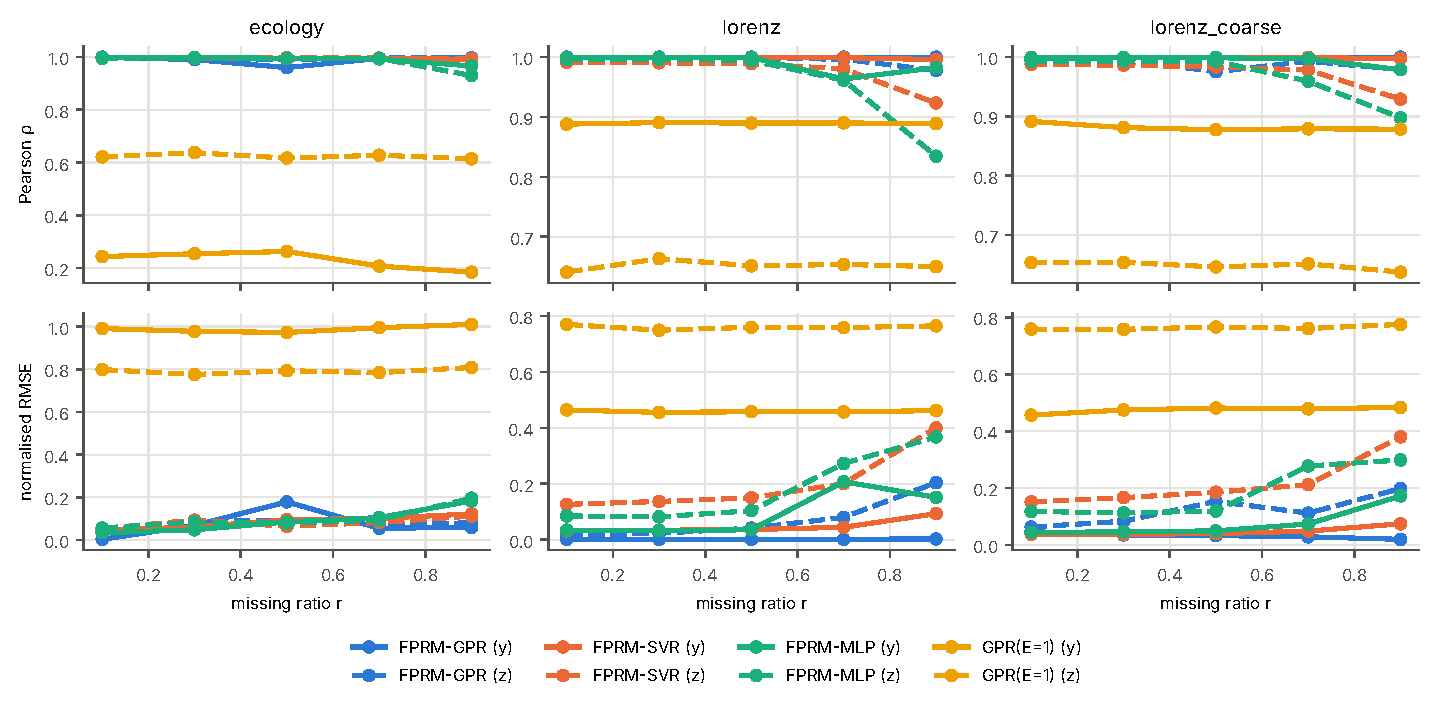
\includegraphics[width=\linewidth]{synthetic_reproduction.pdf}
  \caption{Model-system reproduction versus missing ratio $r$ (solid: $y$, dashed: $z$; 20 repetitions). Top row: Pearson $\rho$; bottom row: normalised RMSE. FPRM with GPR, SVR or MLP mappings stays near $\rho=1$, whereas GPR on the current value of $x$ alone ($E=1$) fails.}
  \label{fig:synthetic}
\end{figure}

\subsection{Overall comparison on PV data}

\Cref{tab:rank} ranks the 17 methods on every (test set, series) pair by RMSE.
\Cref{tab:median} gives the median RMSE, and \cref{fig:curves} shows how RMSE depends on the missing ratio and the gap length.
Four observations stand out.
\begin{enumerate}
  \item In ordinary scenarios (S1--S3), all regression-type methods reach $\rho\approx0.98$. Their RMSE differences of about 1\pct{}cap are therefore invisible to correlation-based evaluation.
  \item In the same scenarios, RF, SVR and MLP on all complete neighbours are the strongest methods (mean ranks 3.6--5.3).
  \item Single-reference FPRM ranks 6.9--7.4 there. It is, however, consistently better than its embedding-free twin FPRM-E1 (ranks 9.6--10.0).
  \item FPRM-multi attains the best overall mean rank (5.7).
\end{enumerate}
Interpolation-type methods (Linear, CSI-Linear, Diurnal) are far behind whenever neighbours are available, and their errors grow quickly with gap length (\cref{fig:curves}b).
Energy errors over removed periods are below 1\pct{} for FPRM and the ML regressors in S1--S3 (Appendix \cref{tab:energy}).

\begin{table}[t]
  \centering\small
  \caption{Mean rank of each method (1 = best of 17) by RMSE (\%cap) per (test set, incomplete series), by scenario. Bold: best per column.}
  \label{tab:rank}
  \input{\tabdir/rank}
\end{table}

\begin{table}[t]
  \centering\small
  \caption{Median daytime RMSE (\% of capacity) over all datasets, seeds and series. In S7, most methods coincide with the CSI-Linear fallback (24.2) because no reference is available. Bold: best per column.}
  \label{tab:median}
  \input{\tabdir/median_rmse}
\end{table}

\begin{figure}[t]
  \centering
  \begin{subfigure}{\linewidth}\centering
    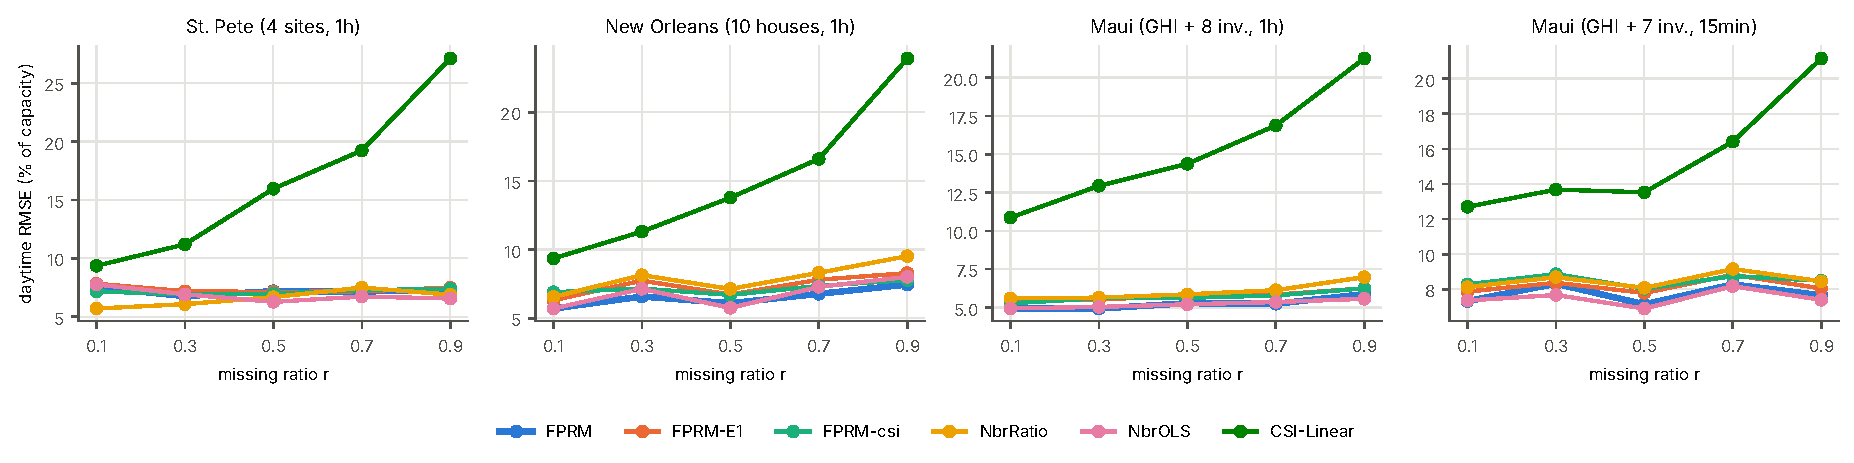
\includegraphics[width=\linewidth]{s1_mcar_curves.pdf}\caption{S1: random missingness, ratio $r$.}
  \end{subfigure}\\[4pt]
  \begin{subfigure}{\linewidth}\centering
    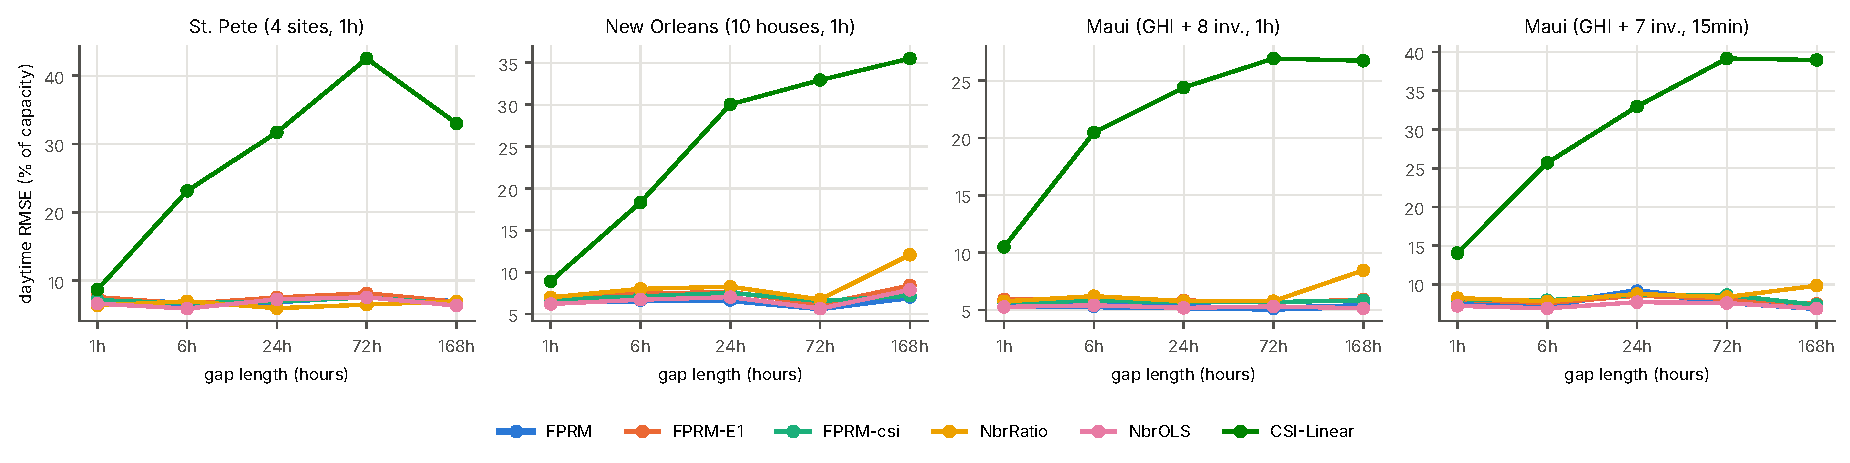
\includegraphics[width=\linewidth]{s2_block_curves.pdf}\caption{S2: contiguous gaps of length $L$ (20\pct{} missing).}
  \end{subfigure}
  \caption{Daytime RMSE (\%cap) of FPRM, its ablations and practitioner baselines on the four datasets (mean over seeds and incomplete series). FPRM is consistently below FPRM-E1, which shows the benefit of embedding, and roughly on par with neighbour regression (NbrOLS). Clear-sky-index interpolation degrades quickly with gap length.}
  \label{fig:curves}
\end{figure}

\subsection{FPRM against the best baseline}

For each (dataset, scenario, parameter) cell we compare FPRM with the best of the 13 non-FPRM methods in that cell (\cref{tab:family,fig:heatmap}).
This per-cell oracle selection is deliberately unfavourable to FPRM; mean ranks (\cref{tab:rank}) give the fixed-method comparison.

In S1--S3, single-reference FPRM is 12--16\pct{} worse in median: it wins 1 of 52 cells and loses 35 significantly.
FPRM-multi is 5--9\pct{} worse in median, wins 18 cells (7 significantly) and loses 15 significantly.
In all scenarios except S4 and S7, FPRM improves on FPRM-E1 by a median 0.5--7.6\pct{}.

\begin{table}[t]
  \centering\small
  \caption{FPRM and FPRM-multi versus the best non-FPRM baseline of each (dataset, scenario, parameter) cell. ``Median rel.'': median relative RMSE difference (negative = FPRM better); significance: paired Wilcoxon $p<0.05$.}
  \label{tab:family}
  \resizebox{\linewidth}{!}{\input{\tabdir/family}}
\end{table}

\begin{figure}[t]
  \centering
  \begin{subfigure}{0.49\linewidth}\centering
    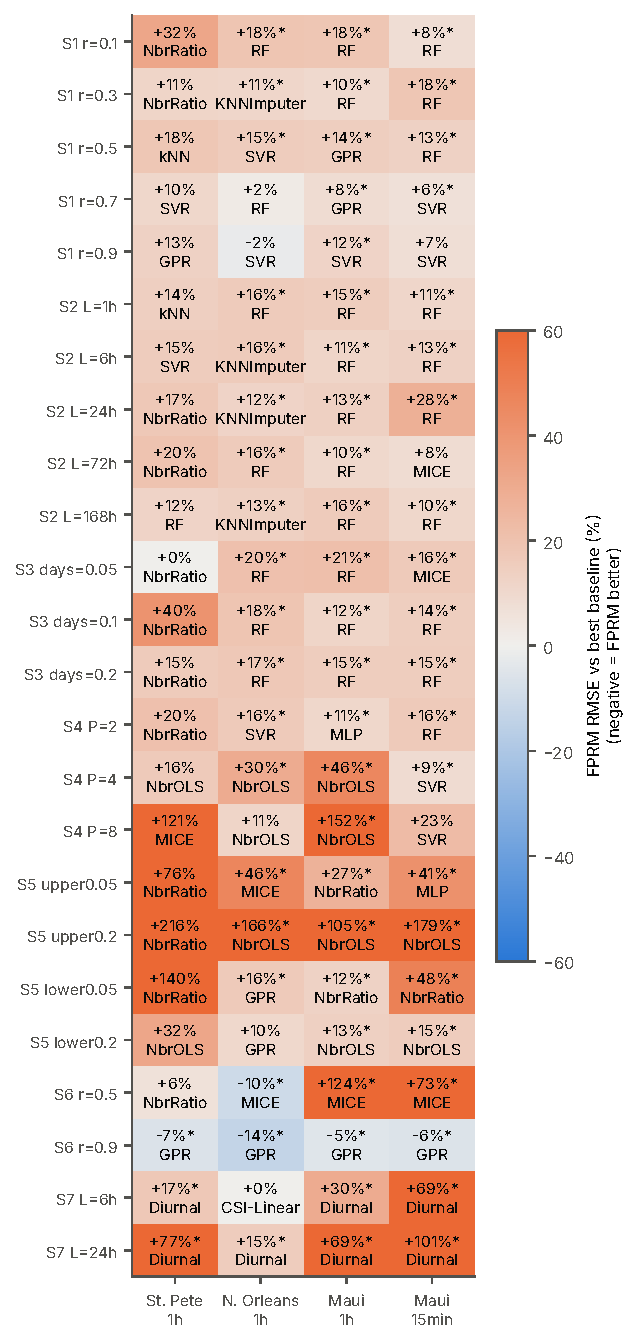
\includegraphics[width=\linewidth]{fprm_vs_best_heatmap.pdf}\caption{FPRM (paper design)}
  \end{subfigure}\hfill
  \begin{subfigure}{0.49\linewidth}\centering
    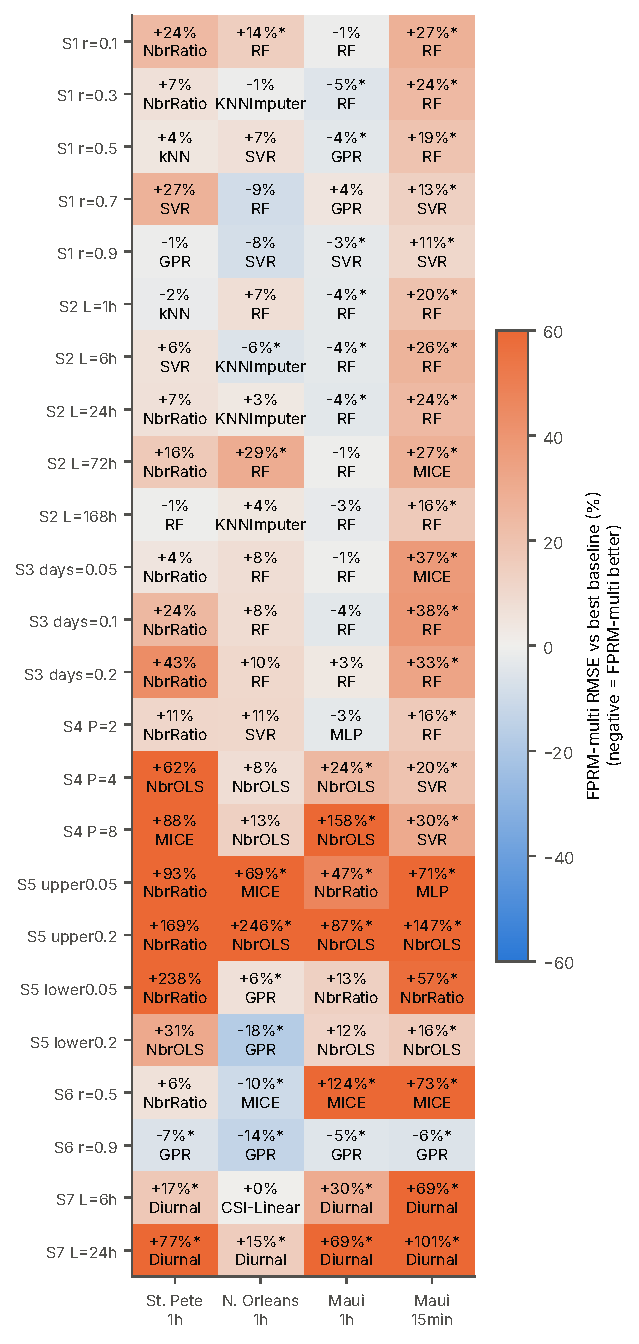
\includegraphics[width=\linewidth]{fprm_multi_vs_best_heatmap.pdf}\caption{FPRM-multi$^\dagger$}
  \end{subfigure}
  \caption{Relative RMSE of FPRM versus the best non-FPRM method of each test cell (blue = FPRM better, orange = worse; $^*$: paired Wilcoxon $p<0.05$; the label names the best baseline). FPRM wins only in S6 at $r=0.9$ and in a few New Orleans cells. Losses concentrate in S4 (periodic), S5 (threshold) and S7 (simultaneous).}
  \label{fig:heatmap}
\end{figure}

\subsection{A single complete series (S6)}

S6 is the regime in which Wu et al.\ report FPRM's largest advantage.
At $r=0.9$, FPRM is the best method on all four datasets, 5--14\pct{} better than the best baseline and significant in every case (\cref{tab:s6,fig:s6}).
When information is scarce, the delay coordinates of the single reference are the most informative input.

At $r=0.5$ the picture changes: MICE wins on Maui by a large margin (7.0 vs.\ 15.7\pct{}cap).
MICE also uses the \emph{partially} observed neighbours at each time step, whereas FPRM only accepts complete series and discards them.
On Maui all methods except MICE are also handicapped because the only complete series is the GHI sensor (\cref{sec:ablation}).
\Cref{fig:example} illustrates S6 reconstructions on clear, overcast and variable days.

\begin{table}[t]
  \centering\small
  \caption{S6 (only the designated reference is complete): RMSE (\%cap), mean over 5 seeds and all incomplete series. Bold: best per row among the listed methods; the last column is the best of all 13 baselines.}
  \label{tab:s6}
  \resizebox{\linewidth}{!}{\input{\tabdir/s6}}
\end{table}

\begin{figure}[t]
  \centering
  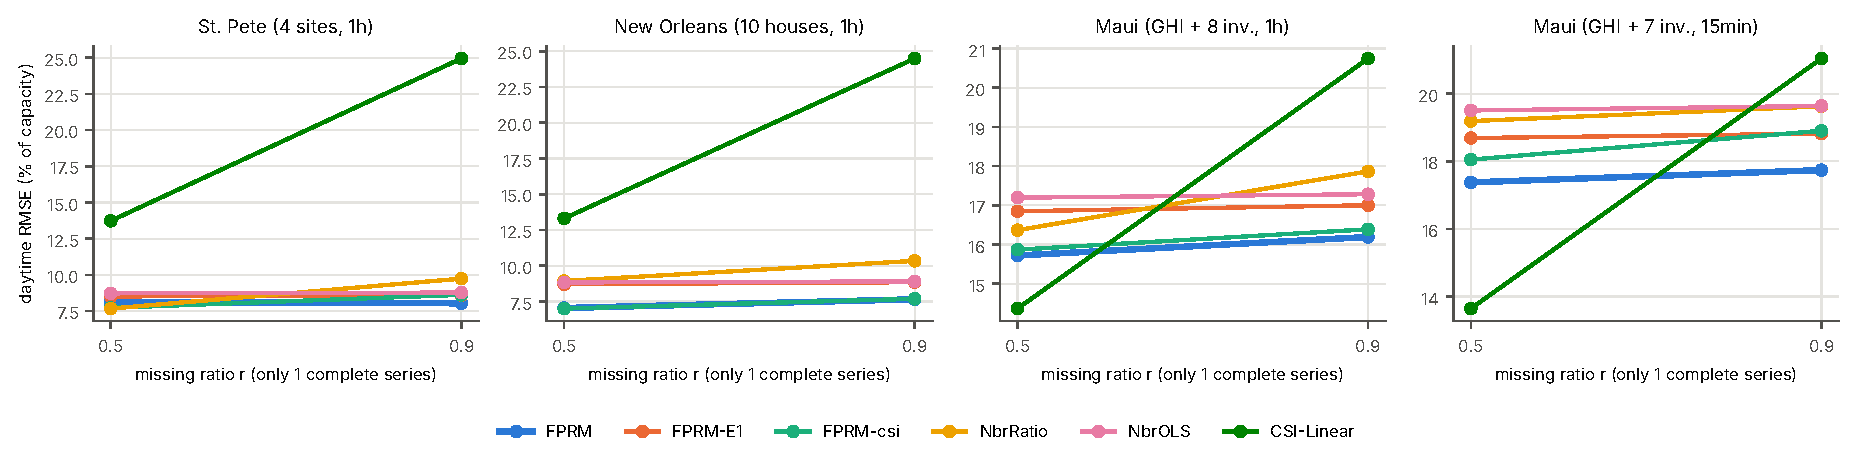
\includegraphics[width=\linewidth]{s6_oneref_curves.pdf}
  \caption{S6: daytime RMSE with a single complete series, at 50\pct{} and 90\pct{} missingness elsewhere. FPRM is lowest at $r=0.9$ on all datasets.}
  \label{fig:s6}
\end{figure}

\begin{figure}[t]
  \centering
  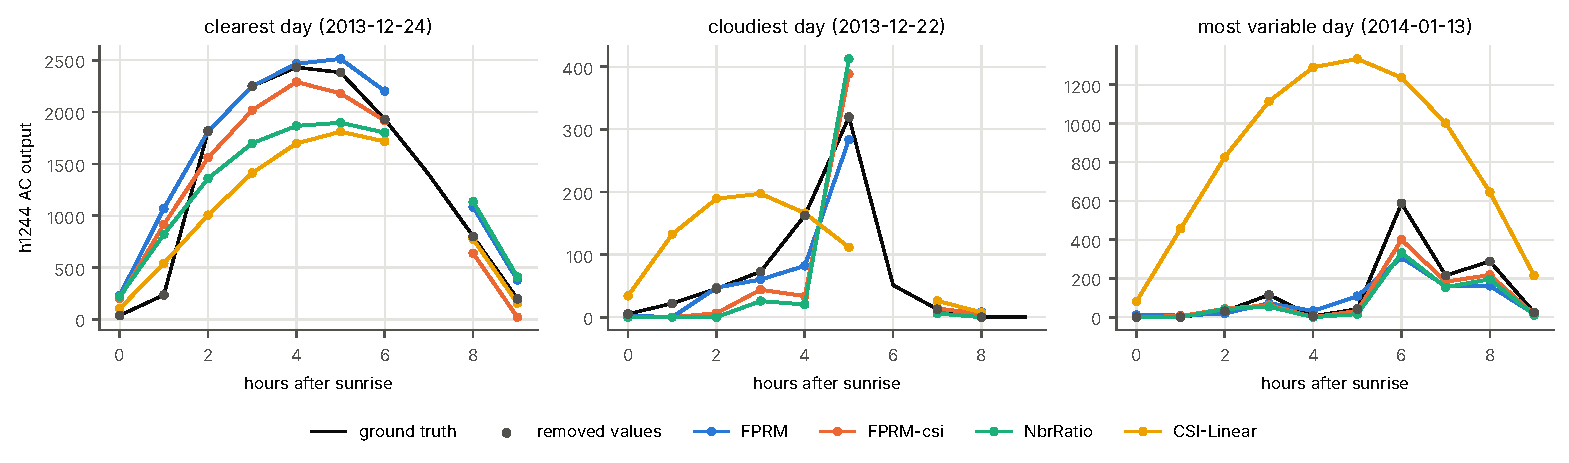
\includegraphics[width=\linewidth]{example_nola_1h_S6_r09.pdf}
  \caption{Example S6 reconstructions (New Orleans, house 1244, $r=0.9$, seed 0) on the clearest, cloudiest and most variable test days. Black: ground truth; dots: removed values; coloured lines: imputations at removed points.}
  \label{fig:example}
\end{figure}

\subsection{Failure modes}\label{sec:failure}

\paragraph{Peak loss (S5, upper).}
When the top 20\pct{} of daytime values are removed, a simple model of saturation or clipping loss, FPRM's RMSE is 12.0--23.3\pct{}cap.
Linear neighbour methods (NbrOLS, NbrRatio) reach 5.9--8.8\pct{}cap.
The training set contains no high-output states, and GPR, like RF, $k$NN and SVR, cannot extrapolate beyond the training range; it shrinks towards the mean.
Proportional (linear) models extrapolate naturally.
FPRM-csi is more robust here (mean rank 5.8), because normalising by clear-sky output makes high-output states less extreme.

\paragraph{Time-of-day aliasing (S4, $P\ge4$).}
Keeping one of every $P$ samples of a 24-step day leaves observations at only a few fixed hours.
Cross-validation within those hours then favours large $E$ and $\tau$, which do not generalise to unobserved parts of the attractor.
For example, on Maui (1\,h, $P=8$) FPRM reaches 14.2\pct{}cap against 8.7 for FPRM-E1 and 5.7 for NbrOLS.
For the same reason the Diurnal baseline has no information for the unobserved slots, which is why its energy error is 100\pct{}.

\paragraph{Simultaneous outages (S7).}
Without any complete reference, FPRM cannot impute, as the original paper acknowledges, and every FPRM variant coincides with its fallback.
The same-slot average of neighbouring days (Diurnal) is the best method here (mean rank 3.9).

\paragraph{Numerical divergence.}
MICE diverged numerically in S4 (RMSE of order $10^{45}$).
For this reason we summarise results with ranks and medians.

\subsection{Ablations and reference choice}\label{sec:ablation}

\Cref{tab:ablation} varies one component at a time.
\begin{itemize}
  \item Replacing GPR by SVR or an MLP barely changes accuracy (8.73 and 8.76 vs.\ 8.67\pct{}cap), consistent with the paper's SVM$^*$/NN$^*$ results. SVR is $\sim$45$\times$ faster.
  \item The causal (backward) embedding is as accurate as the forward one, so FPRM can run online.
  \item The clear-sky-index transform does not help on average.
  \item The largest effect is the choice of reference. In S1/S2, fixing the designated GHI sensor as the reference raises the Maui RMSE from 5.5--7.6 to 16.3--17.7\pct{}cap. The designated neighbour references of New Orleans and St.\ Petersburg cost only 0.3--0.7 points.
\end{itemize}

The S8 sweep (\cref{tab:refsweep}) generalises this.
Embedding improves on FPRM-E1 for \emph{all} 31 references, by 4.8--29.6\pct{}.
FPRM-ref beats NbrRatio for every reference in New Orleans and Maui, but for none in St.\ Petersburg, where the four profiles are nearly proportional.
On Maui, the GHI sensor is the worst reference by far (15.7--17.4\pct{}cap vs.\ 6.2--13.7 with an inverter).

\begin{table}[t]
  \centering\small
  \caption{FPRM ablations (S1 $r\in\{0.5,0.9\}$, S2 $L\in\{6,24\}$\,h, S6 $r\in\{0.5,0.9\}$; 4 datasets, 3 seeds). RMSE in \%cap; time per incomplete series (fit + predict, one CPU core). $^\dagger$: not in the original paper.}
  \label{tab:ablation}
  \input{\tabdir/ablation}
\end{table}

\begin{table}[t]
  \centering\small
  \caption{S8 reference sweep (S6 mask, $r=0.5$, 2 seeds): RMSE (\%cap) range and (mean) over references, mean (min, max) relative gain of FPRM-ref over FPRM-E1, and number of references for which FPRM-ref beats NbrRatio.}
  \label{tab:refsweep}
  \resizebox{\linewidth}{!}{\input{\tabdir/refsweep}}
\end{table}

\section{Discussion}\label{sec:discussion}

\paragraph{Why standard regressors win in ordinary gaps.}
Neighbouring PV series share the cloud field and are correlated at 0.97--0.99.
The instantaneous values of several neighbours therefore already pin down the target state, and the marginal information contributed by delay coordinates of \emph{one} neighbour is smaller than that of additional neighbours.
FPRM-multi, which combines both, recovers most of the gap.
This suggests that the useful content of FPRM for PV is the delay embedding, not the single-reference restriction.

\paragraph{What FPRM discards.}
FPRM requires complete inputs, so a neighbour that is missing even a few values is unusable.
Real fleets rarely lose all neighbours at once.
The S6 $r=0.5$ result, where MICE wins by exploiting partially observed series, indicates the most promising extension: embeddings that tolerate missing coordinates, or an iterative scheme that feeds imputed neighbours back as references.

\paragraph{Physical references are not better references.}
An on-site pyranometer is, intuitively, the most ``physical'' predictor of PV output, yet it was the worst reference.
Differences in plane of array, shading and clock alignment make the pyranometer a poorer proxy of the array state than any inverter on the same roof.
Reference selection should be data-driven, using the observed-period correlation.

\paragraph{Recommended pipeline.}
Gaps should be routed by missingness pattern:
\begin{itemize}
  \item fleet-wide outages: Diurnal or CSI interpolation;
  \item suspected peak or clipping loss: NbrOLS or NbrRatio;
  \item few complete series and heavy missingness elsewhere: FPRM, with SVR, the best-correlated reference and a causal embedding if online;
  \item otherwise: RF/SVR on all complete neighbours, or FPRM-multi, possibly as an ensemble.
\end{itemize}

\section{Limitations}\label{sec:limitations}
\begin{itemize}
  \item \textbf{Data access.} Only NREL PVDAQ data were reachable. Validation on other climates, utility-scale plants and Korean fleets, and against satellite irradiance, remains to be done.
  \item \textbf{Original code.} We could not compare against the authors' MATLAB code or supplementary material, and our Lorenz numbers differ from the paper's.
  \item \textbf{Seeds and windows.} We used five seeds (three for ablations) and windows of five to six months. Year-long series would stress the GPR subset-of-data limit.
  \item \textbf{Embedding selection.} The cross-validated $(E,\tau)$ varies across seeds ($E=2$--8), so selection is a source of variance.
  \item \textbf{Missing extensions.} Lag-FPRM, S-map/MVCM and deep imputers (BRITS, SAITS) were not evaluated.
\end{itemize}

\section{Conclusion}
Dynamics-informed imputation partly transfers to solar PV.
The delay embedding at the core of FPRM consistently improves the same regressor and makes FPRM the best method when only one complete series survives heavy missingness.
In typical PV monitoring, however, several complete neighbours are available.
There, the paper's single-reference design is outperformed by standard regressors on all neighbours, and it fails under peak loss, aliased logging and simultaneous outages.
FPRM is therefore best used as a specialist component, ideally in the multi-reference form, inside a pattern-aware imputation pipeline.

\section*{Data and code availability}
All data are public NREL PVDAQ datasets~\cite{pvdaq} (OEDI, CC BY 4.0).
Code, processed datasets, masks (regenerable), raw results and the scripts that generate every table and figure of this paper are available at \url{https://github.com/jk-60hz/Wu-2026-missing-data}.

\section*{Author contributions and AI disclosure}
J.\ Kim conceived the study, specified the research questions and the evaluation design, and reviewed the results and the manuscript.
Claude Opus 5.5, an AI system developed by Anthropic, carried out the work under J.\ Kim's direction:
\begin{itemize}
  \item implemented FPRM and the benchmark;
  \item acquired and pre-processed the data;
  \item ran all experiments and analysed the results;
  \item drafted the manuscript in English and Korean.
\end{itemize}
All numbers in this paper are generated from the released result files by the released scripts.

\bibliographystyle{unsrtnat}
\bibliography{../refs}

\clearpage
\appendix
\section{Additional results}

\begin{table}[h]
  \centering\small
  \caption{Median absolute error of total energy over removed daytime periods (\% of true energy). Bold: best per column.}
  \label{tab:energy}
  \input{\tabdir/energy}
\end{table}

\begin{table}[h]
  \centering\small
  \caption{Mean rank by dataset (all scenarios). Bold: best per column.}
  \label{tab:rank_ds}
  \input{\tabdir/rank_by_dataset}
\end{table}

\begin{table}[p]
  \centering\scriptsize
  \caption{Daytime RMSE (\%cap) for every scenario and parameter, averaged over datasets, seeds and incomplete series. Bold: best per row; ``div.'': numerical divergence (MICE in S4).}
  \label{tab:full}
  \resizebox{\linewidth}{!}{\input{\tabdir/full}}
\end{table}

\begin{figure}[p]
  \centering
  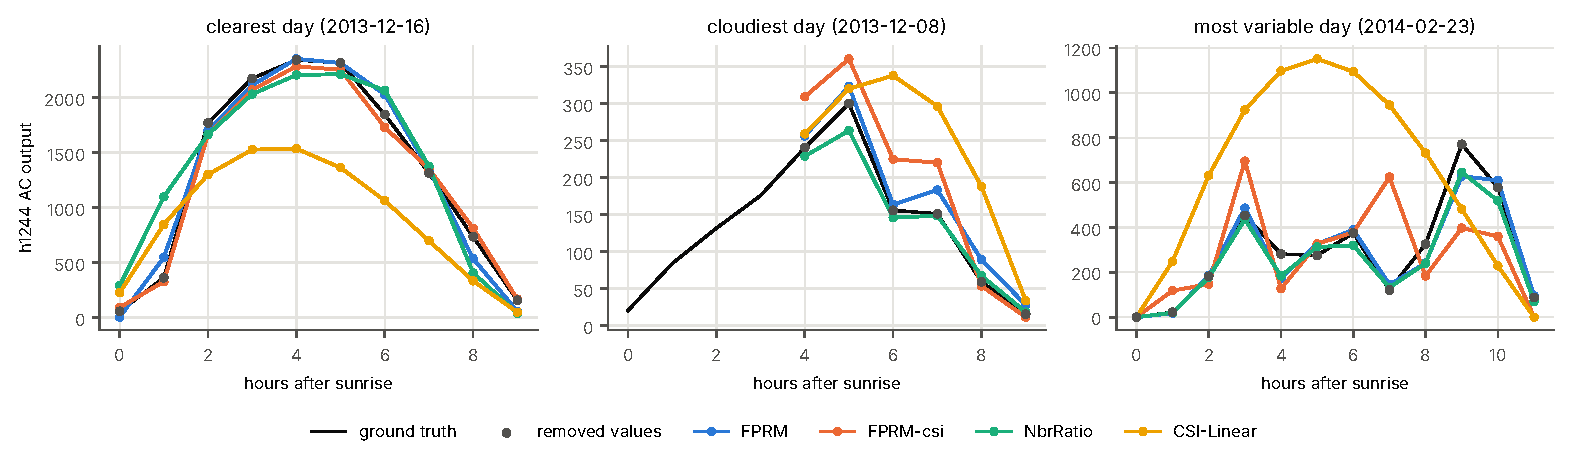
\includegraphics[width=\linewidth]{example_nola_1h_S2_24h.pdf}\\[-1pt]{\small (a) New Orleans, S2 $L=24$\,h}\\[4pt]
  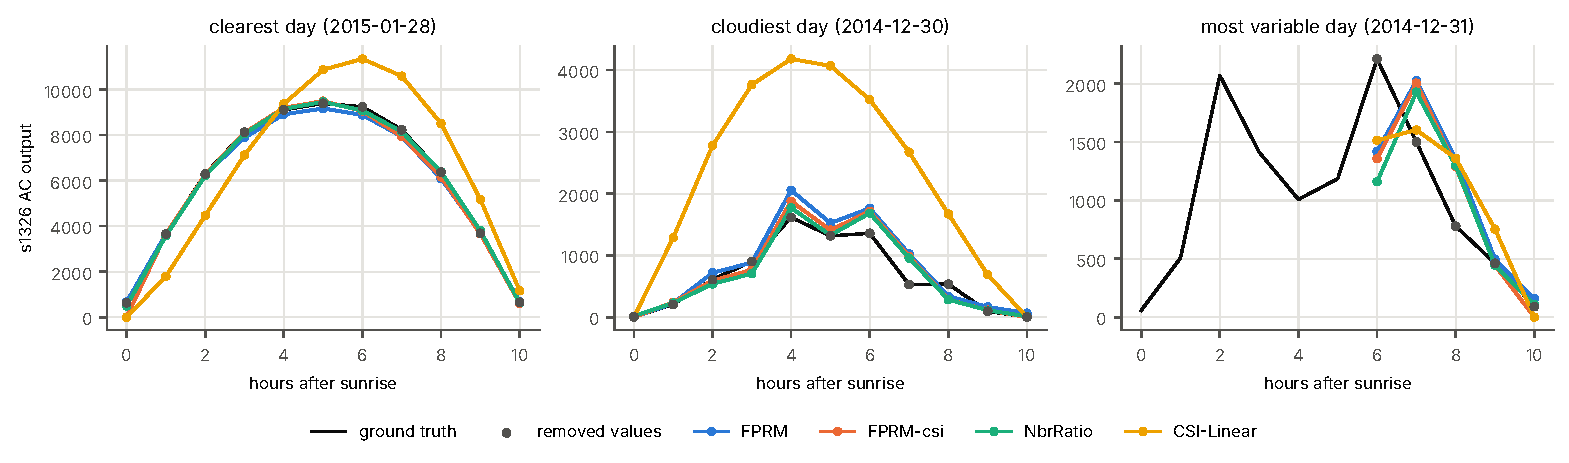
\includegraphics[width=\linewidth]{example_stpete_1h_S2_24h.pdf}\\[-1pt]{\small (b) St.\ Petersburg, S2 $L=24$\,h}\\[4pt]
  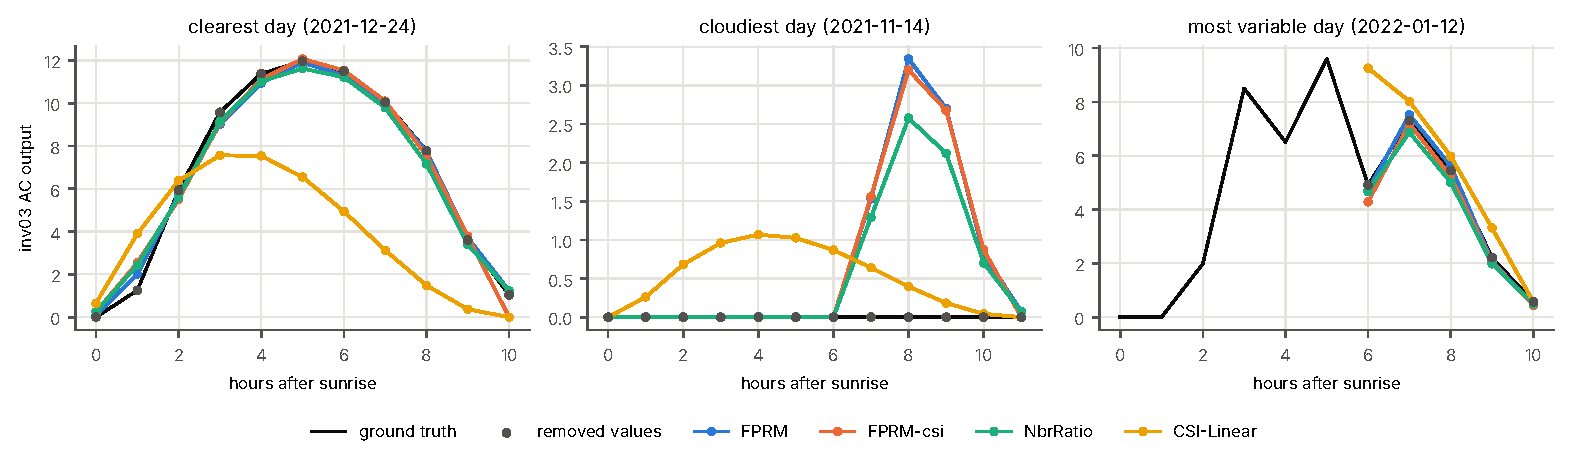
\includegraphics[width=\linewidth]{example_maui_1h_S2_24h.pdf}\\[-1pt]{\small (c) Maui 1\,h, S2 $L=24$\,h}\\[4pt]
  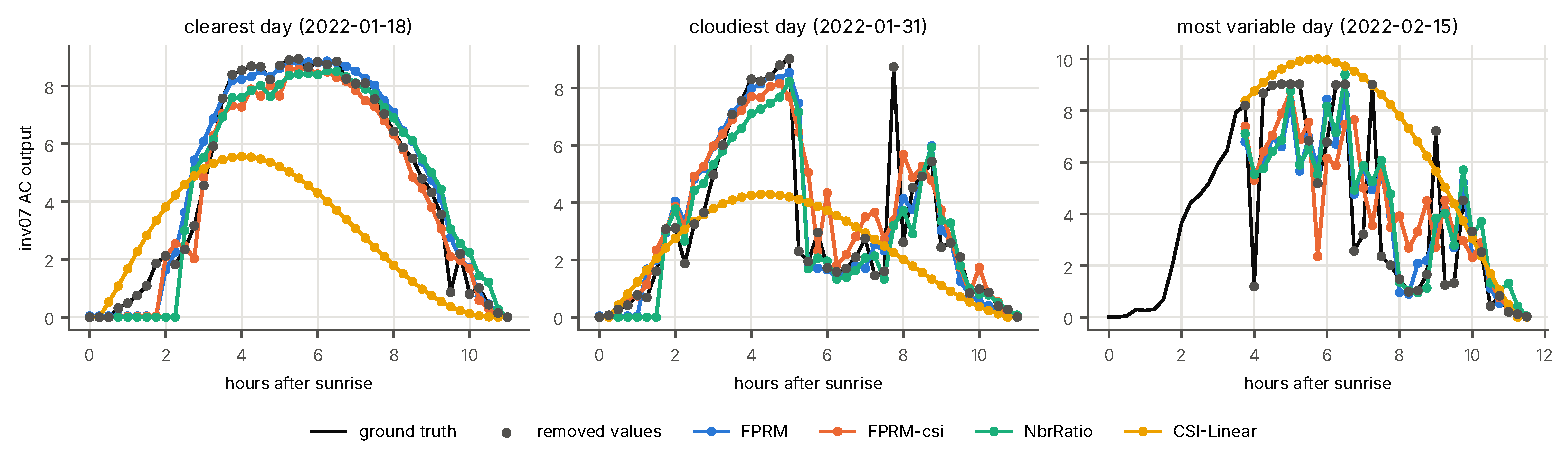
\includegraphics[width=\linewidth]{example_maui_15min_S2_24h.pdf}\\[-1pt]{\small (d) Maui 15\,min, S2 $L=24$\,h}
  \caption{Example reconstructions of 24-h gaps (seed 0, first incomplete series) on the clearest, cloudiest and most variable test day of each dataset.}
  \label{fig:ex_s2}
\end{figure}

\begin{figure}[p]
  \centering
  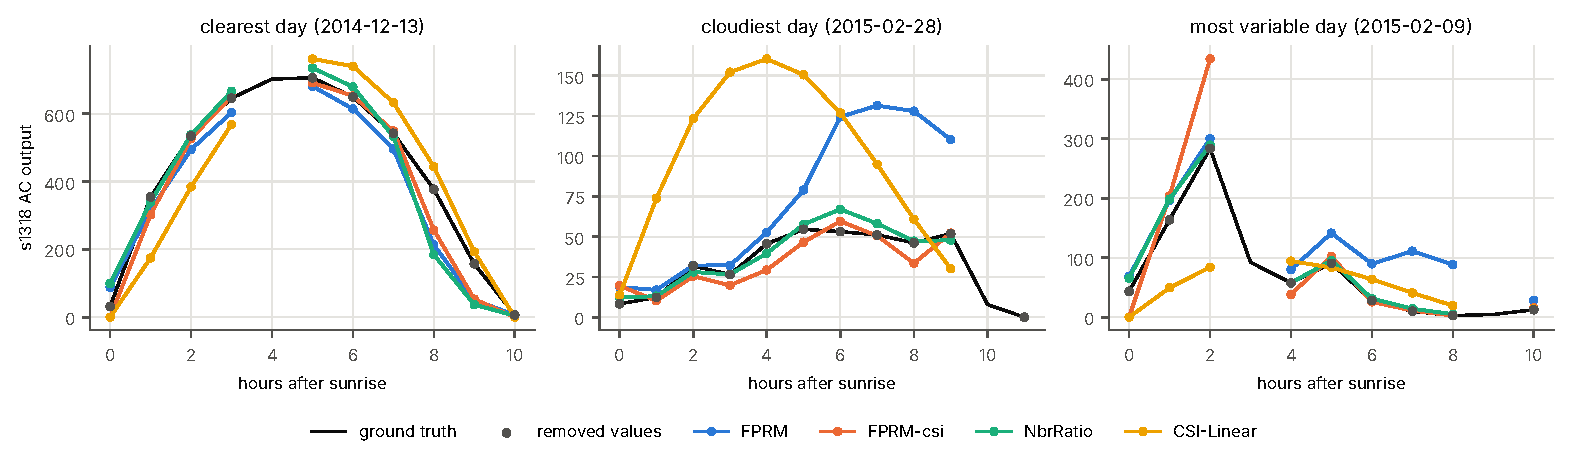
\includegraphics[width=\linewidth]{example_stpete_1h_S6_r09.pdf}\\[-1pt]{\small (a) St.\ Petersburg, S6 $r=0.9$}\\[4pt]
  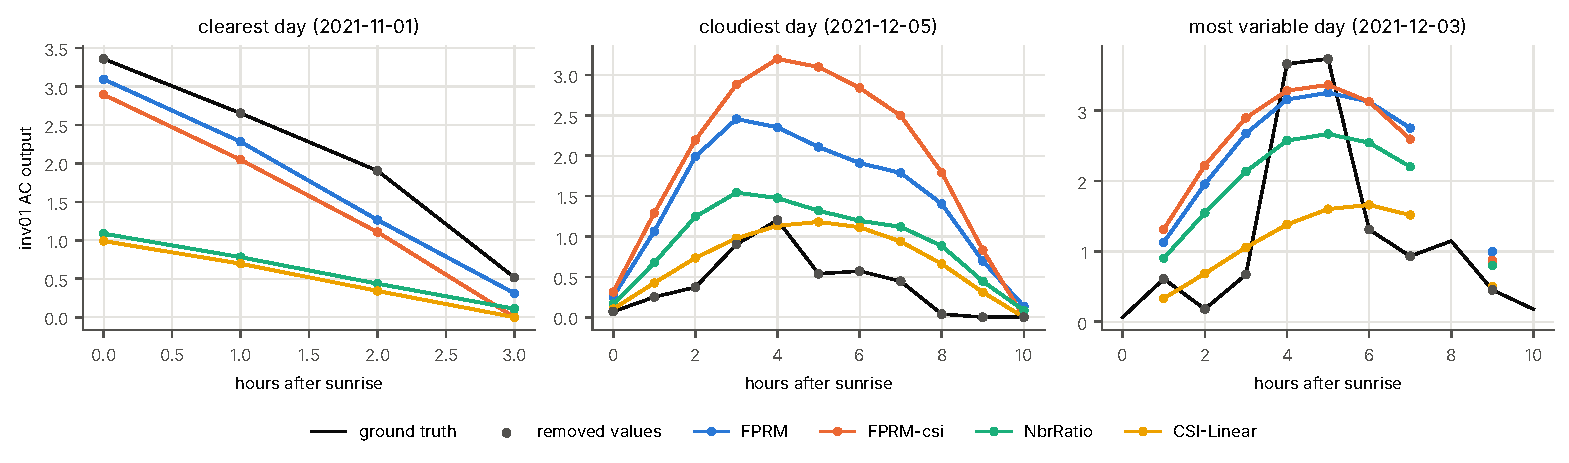
\includegraphics[width=\linewidth]{example_maui_1h_S6_r09.pdf}\\[-1pt]{\small (b) Maui 1\,h, S6 $r=0.9$ (reference: GHI)}\\[4pt]
  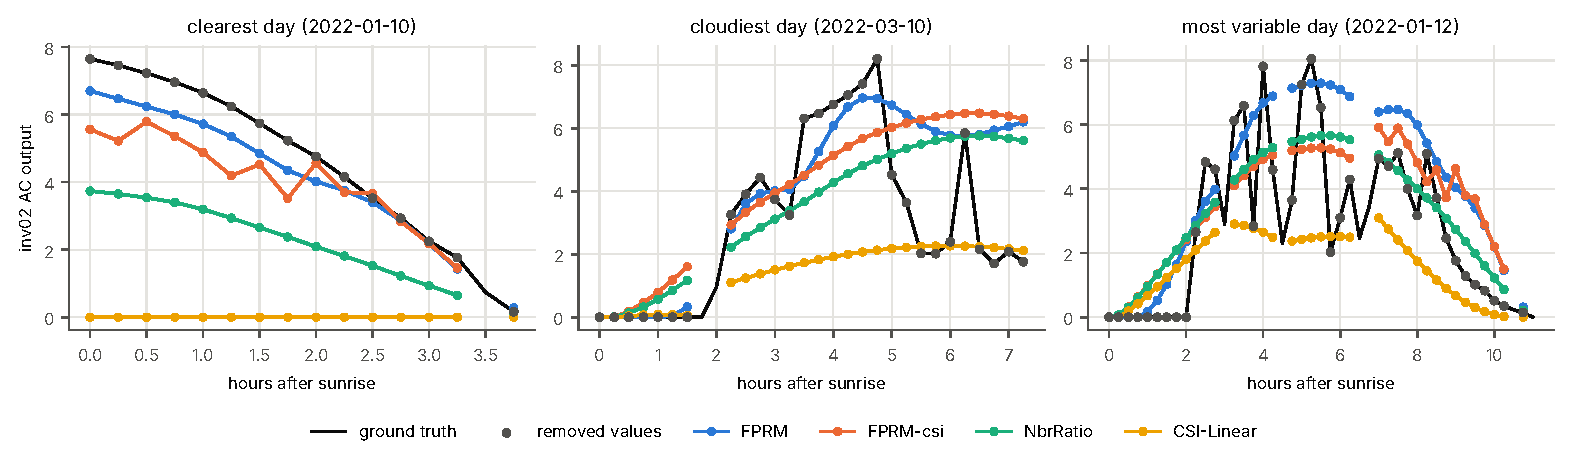
\includegraphics[width=\linewidth]{example_maui_15min_S6_r09.pdf}\\[-1pt]{\small (c) Maui 15\,min, S6 $r=0.9$ (reference: GHI)}
  \caption{Example S6 reconstructions at $r=0.9$ (seed 0, first incomplete series).}
  \label{fig:ex_s6}
\end{figure}

\section{Reproducibility}
{\small\begin{verbatim}
python -m pytest -q tests
python scripts/reproduce_synthetic.py --reps 20 --workers 4
python scripts/make_testsets.py --seeds 5 \
    --datasets maui_15min,maui_1h,stpete_1h,nola_1h
python scripts/run_benchmark.py --config configs/main.yaml
python scripts/run_benchmark.py --config configs/ablation.yaml
python scripts/make_report.py --paper     # figures of this paper
python scripts/make_tables_tex.py         # tables of this paper
\end{verbatim}}
The main benchmark takes about 3\,h and the ablations about 1\,h on four CPU cores.

\end{document}
